\section{Correlation Analysis}\label{res:correlation}

The establishment of a benchmark provided the foundation for investigating the correlation between various zero-cost proxies and the ground truth represented by the validation accuracy. The Spearman Rank Correlation was employed to measure the correlation, as discussed in \cref{sec:corr}. 

\Cref{tab:corr} displays the obtained results, utilising the 693 architectures derived from the created benchmark. 
\clearpage

\begin{table}[h]
\caption{Correlation coefficients between proxy scores and model performance before training}
\centering
\begin{tabular}{lr}
\textbf{Name} & \textbf{$\rho$} \\ \hline
\multicolumn{1}{l|}{\cellcolor{verylightgray}epe\_nas} & \cellcolor{verylightgray}$0.0090$ \\
\multicolumn{1}{l|}{fisher} & $0.2405$ \\
\multicolumn{1}{l|}{\cellcolor{verylightgray}flops} & \cellcolor{verylightgray}$0.7241$ \\
\multicolumn{1}{l|}{grad\_norm} & $0.2653$ \\
\multicolumn{1}{l|}{\cellcolor{verylightgray}grad\_sign} & \cellcolor{verylightgray}$0.4979$ \\
\multicolumn{1}{l|}{grasp} & $-0.4244$ \\
\multicolumn{1}{l|}{\cellcolor{verylightgray}jacov} & \cellcolor{verylightgray}$-0.0465$ \\
\multicolumn{1}{l|}{l2\_norm} & $0.7325$ \\
\multicolumn{1}{l|}{\cellcolor{verylightgray}nwot} & \cellcolor{verylightgray}$0.1214$ \\
\multicolumn{1}{l|}{params} & $0.6164$ \\
\multicolumn{1}{l|}{\cellcolor{verylightgray}plain} & \cellcolor{verylightgray}$0.2490$ \\
\multicolumn{1}{l|}{snip} & $0.2468$ \\
\multicolumn{1}{l|}{\cellcolor{verylightgray}synflow} & \cellcolor{verylightgray}0.7599 \\
\multicolumn{1}{l|}{zen} & \textbf{0.7827} \\
\end{tabular}
\label{tab:corr}
\end{table}

\begin{comment}
\begin{figure}[h!]
  \centering
  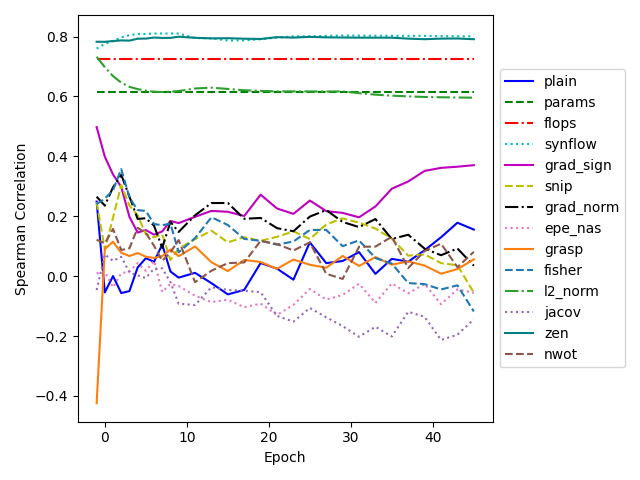
\includegraphics[width=0.8\columnwidth]{figures/correlations.png}
  \caption{Correlations for all zero-cost proxies over multiple epochs}
  \label{fig:warmup}
\end{figure}
\end{comment}


The results in \cref{tab:corr} reveal that specific proxies correlate strongly with the validation accuracy, while others demonstrate weaker correlations. \Cref{tab:corr} indices that Zen has the highest correlation with model performance, with a coefficient of $0.7827$. \gls{Synflow} is also performing well, with a coefficient of $0.7599$. This suggests that both Zen and \gls{synflow} are the most effective zero-cost proxies among the ones considered in this study. 

Conversely, the epe\_nas and jacov proxies exhibit a weak correlation with the model performance, with coefficients of $0.0090$ and $-0.0465$, respectively. 

It is also worth noting that the l2\_norm, \gls{flops}, and params proxies show relatively strong correlations with coefficients of $0.7325$, $0.7241$, and $0.6164$, respectively. Although these proxies might be less effective than Zen and \gls{synflow}, they still demonstrate considerable potential for predicting model performance.

The findings of this correlation analysis provide valuable insights into the predictive capacity of each proxy in relation to the ground truth. This understanding can inform the development of more efficient and effective \gls{NAS} approaches, thereby reducing computational demands and enabling more rapid progress in the field.